\section{Q-values}

\begin{frame} 
\mode<presentation>{
    \begin{center} \huge
        \secname
    \end{center}  
    }
    \begin{center} 
    values of state-action pairs
    \end{center}
\end{frame}

\begin{frame}

\notesonly{
Another measure use for evaluating policies is the state-action value function, also known as the Q-value function.
We can think of the Q-value function as }a ``higher resolution'' value function. \slidesonly{state value $\rightarrow$ state-action value}

\begin{center}
		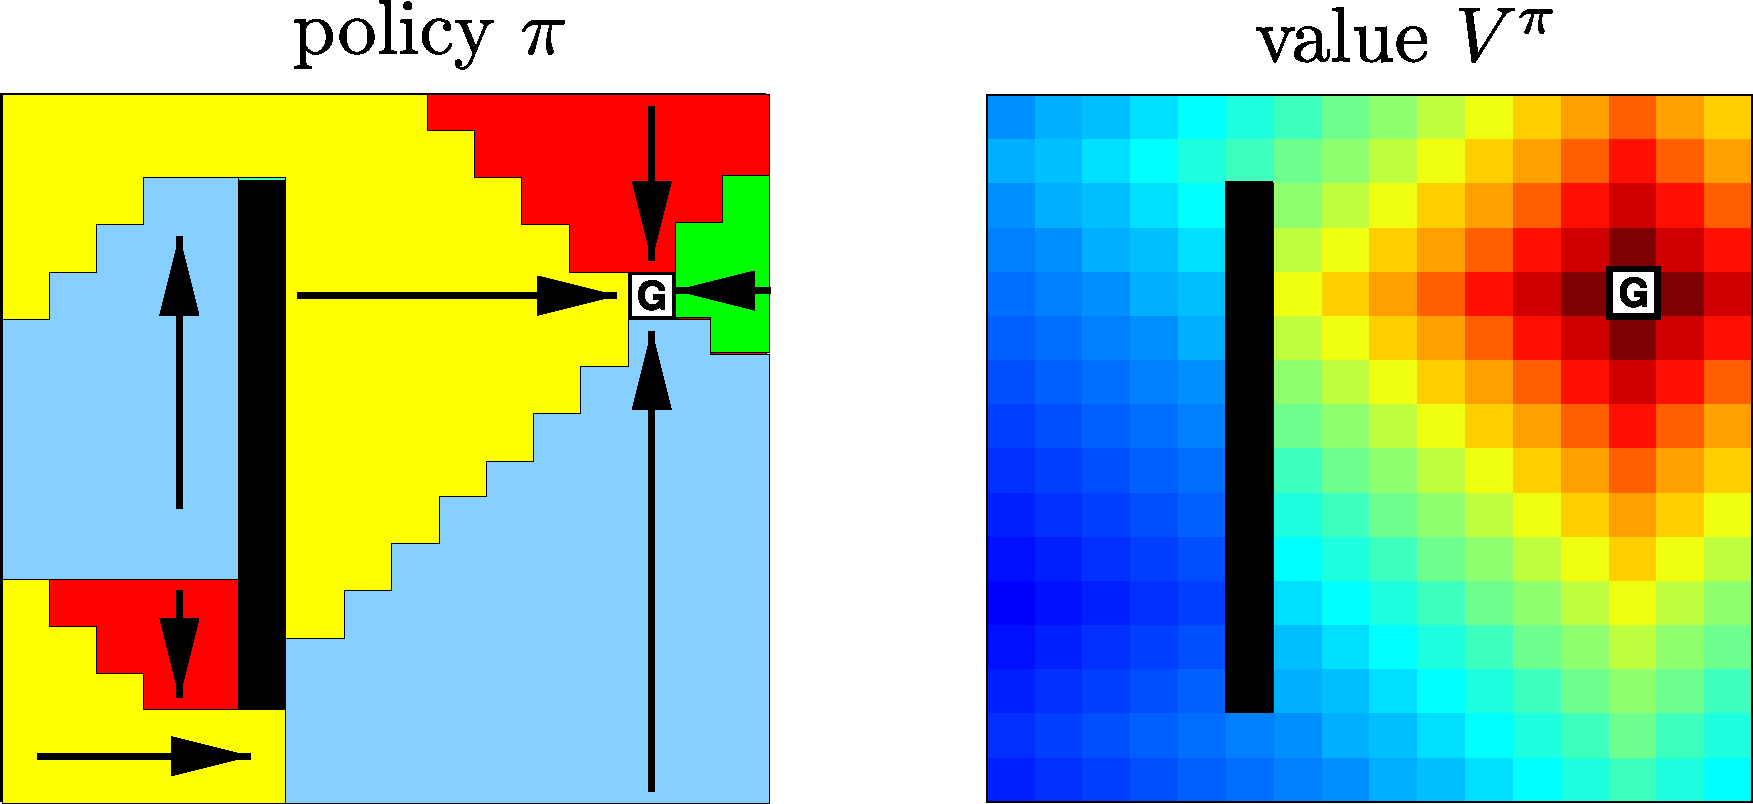
\includegraphics[width=8cm]{img/nav_policy_and_value}
\end{center} 

\begin{center}
		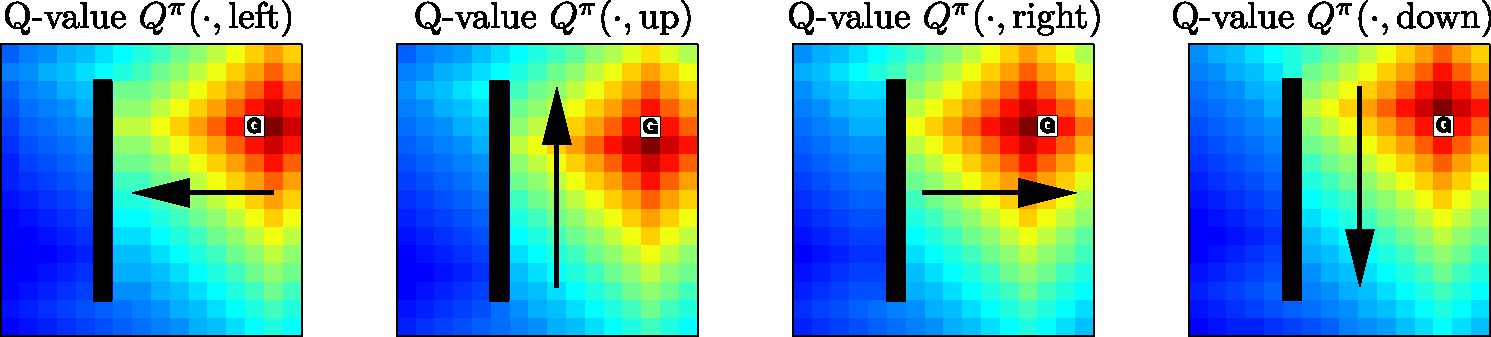
\includegraphics[width=\notesonly{0.9}\textwidth]{img/nav_qvalues}
\end{center} 

\end{frame}

\begin{frame}\frametitle{The Q-value function}

For a fixed policy ${\color{policy}}\pi$, the state-action value function (Q-value function) is defined as:

\begin{equation}
		Q^\pi(\vec x_i, \vec a_k) \quad=\quad 
		\E\bigg\lbrack \,
			\smallsum{t=0}\infty \, \gamma^t \,  
				{\color{reward}r(\vec x^{(t)}, \vec a^{(t)})}
			\, \bigg| \begin{array}{l}
				\scriptstyle \vec x^{(0)} =\, \vec x_i \,, \quad 
					\vec a^{(0)} =\, \vec a_k \\[-1mm]
				\scriptstyle {\color{trans} \vec x^{(t+1)} 
					\,\sim\, P(\cdot|\vec x^{(t)}, \vec a^{(t)})}\\[-1mm]
				\scriptstyle {\color{policy} \vec a^{(t+1)} 
				\,\sim\, \pi(\cdot|{\color{trans}\vec x^{(t+1)}})}
			\end{array}	
		\bigg\rbrack
\end{equation}

The state-action value measures the expected return whenever we start at $\vec x_i$ and take action $\vec a_k$ and follow the policy $\pi$ from there\notesonly{ (cf. \eqref{eq:qbellman})}.

\end{frame}

\begin{frame}

\mode<presentation>{
We have:
\begin{itemize}
\item[] states $\vec x \in \{ \vec x_1, \ldots, \vec x_S\}$, 
actions $\vec a \in \{ \vec a_1, \ldots, \vec a_A\}$,\\
reward function $r(\vec x_i, \vec a_k)$,
\item[]
transition model ${\color{trans} P(\vec x_j | \vec x_i, \vec a_k)}$ and
policy ${\color{policy} \pi(\vec a_k | \vec x_i)}$
\end{itemize}
}

\mode<presentation>{
\begin{center}
		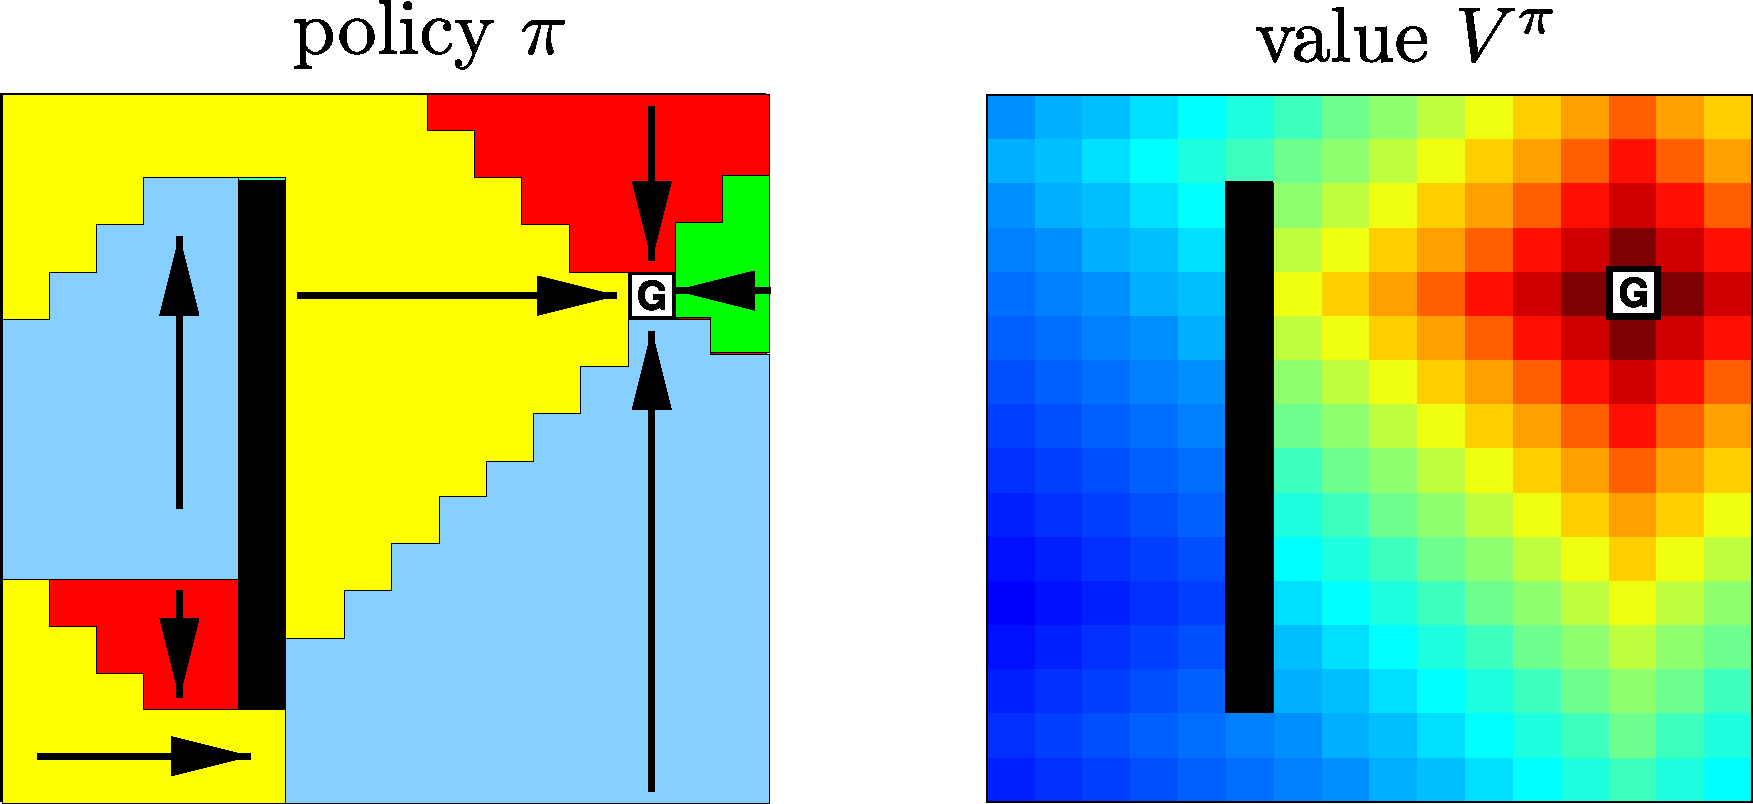
\includegraphics[width=3cm]{img/nav_policy_and_value}
\end{center} 

\begin{center}
		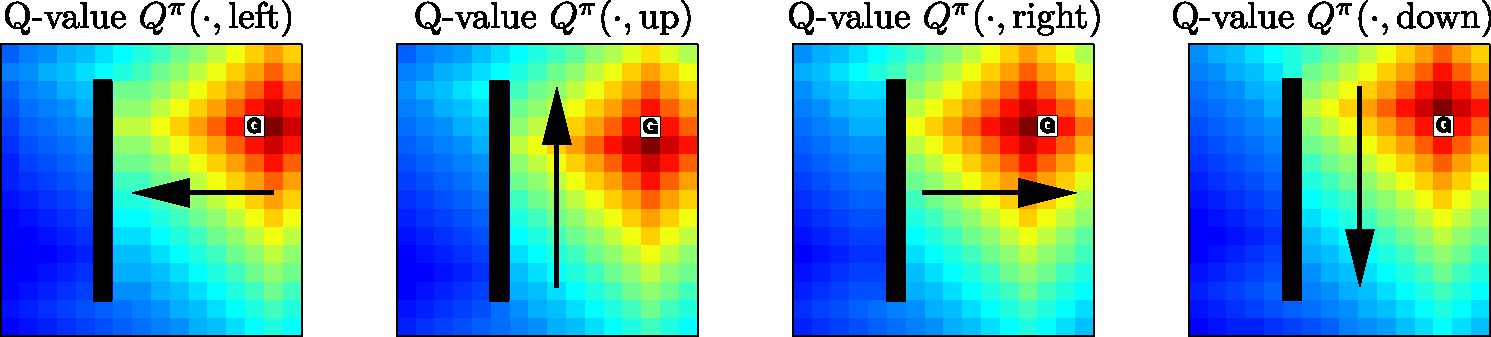
\includegraphics[width=0.7\textwidth]{img/nav_qvalues}
\end{center} 
}

\question{How does the value function relate to the Q-value function?}

\pause

\slidesonly{\vspace{-7mm}}
\notesonly{- yes, through:}

\begin{equation}
V^\pi(\vec x_i) = \visible<3->{
{\only<4>{\color{policy}}\sum_{k=1}^{A}}
}
\visible<4>
{{\color{policy}
\pi(\vec a_k|\vec x_i)
}}
\visible<2->{{\color{black}Q^\pi(\vec x, \vec a_k)}}
\label{eq:vfromq}
\end{equation}

\end{frame}

\begin{frame}
	\only<1,2>{
	\begin{block}{Reminder: Bellman equation (decomposition) for the value function}
			\begin{equation}
			V^\pi_i
			= {\color{reward}\vec r^\pi_i} 
					+ \gamma {\color{trans}\vec P^\pi_{ij}} \vec v^\pi_{j}
			\end{equation} 
	\end{block}
	
	\mode<presentation>{
	Knowing that:\\
	
	Q-values measure the expected return whenever we start at $\vec x_i$ and take action $\vec a_k$ and follow the policy $\pi$ from there
	}
	
	\question{Can we get a similar decomposition for the Q-value function?}
	}
	
	\pause
	
	\begin{block}{Bellman equation (decomposition) for Q-values}
		\vspace{-4mm}	
		\begin{align}
			\label{eq:qbellman}
			Q^\pi(\vec x_i, \vec a_k) \;\;&=\;\; 
			{\color{reward} r(\vec x_i, \vec a_k)} \;+\; 
			\gamma {\color{trans} \sum_{j=1}^S 
				P(\vec x_j | \vec x_i, \vec a_k)} \;
				V^\pi({\color{trans}\vec x_j})
			\slidesonly{\\}
			\notesonly{\intertext{plugging \eqref{eq:vfromq} yields:}}
			&=\;\; 
			{\color{reward} r(\vec x_i, \vec a_k)} \;+\; 
			\gamma {\color{trans} \sum_{j=1}^S 
				P(\vec x_j | \vec x_i, \vec a_k)} \;
				{\color{policy} \sum_{l=1}^{A} \, 
					\pi(\vec a_l | {\color{trans}\vec x_j})} \,
					Q^\pi({\color{trans}\vec x_j}, 
						{\color{policy}\vec a_l})
		\end{align}
	\end{block}
	
	\slidesonly{\vspace{-3mm}}
	
	\notesonly{
	Applying the Bellman decomposition to the Q-value function reveals how Q-values relate to the state-value function.
	}
	
	\only<3->{
	
	\question{What are the implications of having the Bellman decomposition for the Q-value function?}
	
	\pause
	
	- \notesonly{It implies that we can reuse the same policy evaluation methods as we did for the value function that directly operate on the Bellman decomposition (e.g. }model-based methods: analytical solution, fixed-point iteration\notesonly{)}\slidesonly{ for finding the q-value function for some policy}
	
	\question{Can I only reuse model-based evaluation methods to estimate Q-values?}
	
	\slidesonly{\vspace{-3mm}}
	
	- \underline{all} techniques for value estimation apply to Q-values.
	}
	
\end{frame}


\subsection{Finding the optimal policy (recap and extension)}

\subsubsection{Comparing two policies}

\begin{frame}\frametitle{My policy is better than yours (recap)}

\begin{equation}
\pi~
\overset{\mathclap{\substack{%
					\text{``better'' or}\\[1mm]\text{equally ``good''}\\ \big\downarrow
					}}}{{\color{gray}\ge}}
~\pi' 
\quad \text{\textbf{iff}} \quad V^{\pi} (\vec x) \ge V^{\pi'} (\vec x)\,,\quad \forall\; \vec x \in \mathcal{X}
\end{equation}

\end{frame}

\begin{frame}\frametitle{\subsecname}

Recall:
\slidesonly{\vspace{-5mm}}
\begin{equation}
V^{*}(\vec x) = \max_{\pi} V^{\pi} (\vec x)\,,\quad \forall\; \vec x \in \mathcal{X}
\end{equation}

\visible<2-4>{
Similarly for state-action values:

\slidesonly{\vspace{-3mm}}

\begin{equation}
Q^{*}(\vec x, \vec a) = \max_{\pi} Q^{\pi} (\vec x, \vec a)\,,\quad \forall\; \vec x \in \mathcal{X}, \vec a \in \mathcal{A}
\end{equation}
}

\slidesonly{\vspace{-3mm}}

\begin{block}{Optimal Policy}

For all optimal policies $\pi^{*}$:

\slidesonly{\vspace{-3mm}}

\begin{equation}
    V^{\pi^{*}}(\vec x) = V^{*}(\vec x) = \max_{\pi} V^{\pi} (\vec x)\,,\quad \forall\; \vec x \in \mathcal{X}
\end{equation}

A policy $\pi$ that maximizes the value function and yields $\vec v^{*}$ is an optimal policy $\pi^{*}$.\visible<3->{ Consequently, $\forall\; \vec x \in \mathcal{X}, \vec a \in \mathcal{A},$

\only<4>{
\slidesonly{\vspace{-7mm}}
}

\begin{align}
    Q^{\pi^{*}}(\vec x, \vec a) 
    = Q^{*}(\vec x, \vec a) &= \max_{\pi} Q^{\pi} (\vec x, \vec a)\\
    \visible<4>{
    &
    %\kern-2e4\stackrel{\notesonly{\text{with}~\eqref{eq:qbellman}}}{=}
    \overset{\mathclap{\substack{%
    \notesonly{\text{with \eqref{eq:qbellman}}}\vspace{3mm}
					}}}{=}
    {\color{reward} r(\vec x_i, \vec a_k)} \;+\; 
			\gamma {\color{trans} \sum_{j=1}^S 
				P(\vec x_j | \vec x_i, \vec a_k)} \;
				V^*(\vec x_j)
				}
\end{align}


}
    
\end{block}

    
\end{frame}

\begin{frame}\frametitle{Optimal state-action value}

\mode<presentation>{
\begin{equation}
Q^{*}(\vec x, \vec a) = \max_{\pi} Q^{\pi} (\vec x, \vec a)\,,\quad \forall\; \vec x \in \mathcal{X}, \vec a \in \mathcal{A}
\end{equation}
}

\question{How do we interpret $Q^{*}(\vec x, \vec a)$?}\\

\pause

- $Q^{*}(\vec x, \vec a)$ gives us the right action to take to behave optimally in the MDP.

\question{Anything else? How do we extract the policy from the state-action values?}\\

\notesonly{
- Simple readout:
}

\begin{equation}
\pi(\vec a_k | \vec x_i) = \visible<3>{\argmax_{\vec a} Q(\vec x_i, \vec a)}
\end{equation}

\question{Any disadvantages to finding the Q-values directly instead of the value function?}\\

\notesonly{
- The space of the Q-values is proportional to the state space \textbf{as well as} the action space. For a large action space the space of the Q-values would be much larger than that of the state value function.
}

\end{frame}

\subsection{\notesonly{On-policy} TD learning of Q-values (SARSA)}

% -----------------------------------------------------------------------------
\begin{frame}\frametitle{\subsecname}
	\begin{itemize}
		\item Online learning requires sampling from a long Markov chain:\\
		\begin{center}
			(State$^{(t)}$-Action$^{(t)}$-{\color{reward} Reward$^{(t)}$}-{\color{trans} State$^{(t+1)}$}-{\color{policy} Action$^{(t+1)}$})
		\end{center}
		\vspace{2mm}
		\item This enables the asynchronous on-line update of the value function one state at a time (cf. TD($0$)\notesonly{ in \eqref{eq:tdlearningvalue}}):
		
		\slidesonly{\vspace{-7mm}}
		
		\begin{equation}
			\tilde V^{\pi}_{(t+1)}(\vec x^{(t)}) \quad = \quad 
			\tilde V^{\pi}_{(t)}(\vec x^{(t)}) \;+\;
			\lr \Big( \underbrace{{\color{reward}r^{(t)}} 
			+ \overbrace{
			\gamma \tilde V^{\pi}_{(t)}({\color{trans}\vec x^{(t+1)}})
			}^{\substack{\text{discounted value of}\\ \text{the next step}}} 
			- \tilde V^{\pi}_{(t)}{(\vec x^{(t)})}}_{\text{TD-error }\Delta V_{(t)}} \Big) 
		\end{equation}
		
		\slidesonly{\vspace{-3mm}}
	
		Applying TD learning to Q-values leads to:
		
		\slidesonly{\vspace{-4mm}}
	
		\begin{align}
			\tilde{Q}^\pi_{(t+1)}(\vec x^{(t)},\, \vec a^{(t)} ) &\\
			 = \, \tilde{Q}^\pi_{(t)} ( \vec x^{(t)},\, \vec a^{(t)} )& \, + \, \eta \, \underbrace{ \big( {\color{reward} r^{(t)}} \, + \, \gamma \, \tilde{Q}^\pi_{(t)} ({\color{trans}  \vec x^{(t+1)}},\,{\color{policy}  \vec a^{(t+1)}} ) - \tilde{Q}^\pi_{(t)} ( \vec x^{(t)},\, \vec a^{(t)} ) \big)}_{\Delta Q_{(t)}}
		\end{align}
		
		\slidesonly{\vspace{-3mm}}
		
		\item There exists a SARSA($\lambda$) variant with eligibility traces (cf. TD($\lambda$)).
	\end{itemize}

\end{frame}

% -----------------------------------------------------------------------------
\begin{frame} \frametitle{On-policy vs. off-policy estimates}
	\begin{block}{On-policy:}
		Q-values are estimated for the policy, which generates the Markov chain.
	\end{block}
	
	\vspace{5mm}
	
	\begin{block}{Off-policy:}
		Q-values are estimated for a policy $\pi$. The Markov chain is generated by a different policy $\pi'$.
	\end{block}
	
	\mode<presentation>{
	SARSA:
	\begin{align}
			\tilde{Q}^\pi_{(t+1)}(\vec x^{(t)},\, \vec a^{(t)} ) &\\
			 = \, \tilde{Q}^\pi_{(t)} ( \vec x^{(t)},\, \vec a^{(t)} )& \, + \, \eta \, \underbrace{ \big( {\color{reward} r^{(t)}} \, + \, \gamma \, \tilde{Q}^\pi_{(t)} ({\color{trans}  \vec x^{(t+1)}},\,{\color{policy}  \vec a^{(t+1)}} ) - \tilde{Q}^\pi_{(t)} ( \vec x^{(t)},\, \vec a^{(t)} ) \big)}_{\Delta Q_{(t)}}
	\end{align}
	}
	
	SARSA estimates the Q-values for a fixed ploicy which generates the Markov chain. Therefore, SARSA is on-policy
\end{frame}

\subsection{Off-policy TD learning of Q-values}

% -----------------------------------------------------------------------------
\begin{frame}{Only} \frametitle{\subsecname}
	
	TD learning of Q-values in general:
	\begin{equation}
			\tilde{Q}^\pi_{(t+1)}(\vec x^{(t)},\, \vec a^{(t)} )
			\,= \,
			\tilde{Q}^\pi_{(t)} ( \vec x^{(t)},\, \vec a^{(t)} ) \, + \, \eta \, {\color{magenta}\Delta Q_{(t)}}
	\end{equation}
	
	\only<1>{
	When going from on to off-policy, what changes is that the actions that lead to the next state are sampled using a \textbf{different} \emph{sampling} policy $\pi'$\\
		\begin{equation}
		\vec a^{(t)} \sim \pi'(\vec a | \vec x^{(t)})
		\end{equation}
		}
	
	\notesonly{In the case of TD learning, on- or off-policy becomes apparant from ${\color{magenta}\Delta Q_{(t)}}$:}
	
	\begin{itemize}
		\item<only@2> On-policy TD learning of Q-values (SARSA):
		
		\begin{equation}
				{\color{magenta}\Delta Q_{(t)}} \,=\, {\color{reward} r^{(t)}} \, + \, \gamma \, \overbrace{\tilde{Q}^\pi_{(t)} ({\color{trans}  \vec x^{(t+1)}},\,{\color{policy}  \vec a^{(t+1)}} )}^{\circledast} - \tilde{Q}^\pi_{(t)} ( \vec x^{(t)},\, \vec a^{(t)} )
				\label{eq:deltaqONpolicy}
		\end{equation}
		
		\item<only@2,3> Off-policy TD learning of Q-values:
		
		\slidesonly{\vspace{-5mm}}
		
		\begin{equation}
					{\color{magenta}\Delta Q_{(t)}} \,=\, {\color{reward}r^{(t)}} 
				 \, + \, \gamma \, \overbrace{{\color{policy}\smallsum{k=1}{A}
					\pi(\vec a_k \,|\, {\color{trans}\vec x^{(t+1)}})} \,
					Q({\color{trans}\vec x^{(t+1)}}, {\color{policy}\vec a_k})}^{\circledast} 
				\;-\; Q(\vec x^{(t)}, \vec a^{(t)})
				\label{eq:deltaqOFFpolicy}
		\end{equation}
		
		The $\circledast$ represents the discounted value of the next step\notesonly{ in both \eqref{deltaqONpolicy} and \eqref{deltaqOFFpolicy}}.
		
		\notesonly{What is happening \eqref{eq:deltaqoffpolicy} is that the discounted value\notesonly{\footnote{in this particular case, the value is the state-action value, but TD learning can be applied to etimating the state value function just as well.}} of the next step is weighted by the probability of the action being sampled by the policy $\pi$ which is being evaluated as it may differ from the sampling policy $\pi'$.}
		
	\item<only@3> Advantage of off-policy: Data (i.e. Markov chains) can be reused as the policy ${\color{policy}\pi}$, the one we want to opitimize, changes (e.g. policy iteration)
	\item<only@3> contracts for ergodic Markov chain, i.e.
	\begin{equation}
	\lim\limits_{p\to\infty} \E\Big\lbrack
				\smallsum{t=0}{p} \Delta Q_{(t)} 
			\Big\rbrack= Q^{\pi}
	\end{equation}
	
	\end{itemize}
	
\end{frame}



